\chapter{基于预测的容器弹性服务策略 }\label{chap:elastic_service}

\section{引言}

在本文前面的章节中,设计了基于容器化的多终端协同服务系统,将位于用户终端边缘的多个智能终端设备上的空余资源整合起来,以容器的形式为用户终端提供服务,以提高终端资源的利用率,提高终端用户的体验。但是在智能终端上以容器的形式对外提供服务的时候,会出现一组矛盾的问题。如果采用预部署的形式,即在边缘终端上提前部署好提供服务的容器,那么收到用户的服务请求就可以马上对外提供服务。但由于智能终端的资源是有限的,终端服务不能像云端系统服务那样一直在后台运行,等待着用户请求流量的到达。这种预部署的方式使得提供服务的容器也会·消耗智能终端上面的资源,在用户请求流量较低的时候会造成一种智能终端资源的浪费。如果采用非预部署的形式,即不提前部署容器,而是等到用户请求到达服务终端以后再临时创建容器提供服务,在服务完成后可以看情况销毁容器,这样就可以减小很多额外开销,节约智能终端的资源。但是这种非预部署的形式会大大增加用户的平均等待时间,因为相比一次服务的计算和网络传输开销,一次容器创建的时间还是非常长的,对于等待服务请求响应的用户来说完全不能够接受。

为了解决多终端协同服务技术中的预部署问题,促进提高终端资源利用率和降低用户服务请求响应等待时间之间的平衡,我们提出基于预测的容器弹性服务策略,根据预测结果提前弹性部署容器服务,动态调整多终端协同服务的规模,平衡提高终端资源利用率与降低用户服务请求响应等待时间之间的关系。本章提出的基于预测的容器弹性服务策略,具体实现为第\ref{chap:service_system}章中所提出的系统架构设计中的弹性服务模块。

本章的内容组织结构如下:第\ref{sec:elastic_service_related_work}节介绍了预测算法的相关研究工作,包括基于统计学模型的预测算法和基于卡尔曼滤波的预测算法;第\ref{sec:elastic_service_Kalman_filtering}节介绍了多终端协同服务中的用户流量预测模型,以及卡尔曼滤波预测算法,并结合多终端协同服务技术场景的特点,提出一种改进的卡尔曼滤波预测算法;第\ref{sec:elastic_service_strategy}节介绍了基于预测的容器弹性服务策略的设计思路,对具体弹性服务策略的流程进行了设计;第\ref{sec:elastic_service_experiment_results}节列出了仿真实验的结果及分析;第\ref{sec:elastic_service_summary}节总结了本章内容。

\section{相关工作}\label{sec:elastic_service_related_work}

\subsection{早期网络流量预测算法}

网络流量的可预测性在许多领域都具有重要意义,包括自适应应用,拥塞控制,准入控制和网络带宽分配等。流量预测需要准确的流量模型,可以捕获实际流量的统计特征\cite{feng2005study}。

早期的网络流量预测算法研究主要是基于线性预测模型的短相关模型,典型的如基于泊松模型、马尔可夫过程及增量高斯混合模型,以及在这些统计学模型的基础上加以改进的一些线性预测模型,例如IPP模型、MMPP模型、MMFM模型等等\cite{2013基于时间相关的网络流量建模与预测研究}。但是由于真实网络环境中的网络流量数据拥有长相关、自相似性、突发性等特点,使用传统的泊松模型、马尔可夫模型等随机模型不能够很好地对网络流量数据进行模拟和预测\cite{段智彬2009基于}。

自回归滑动平均模型(Auto-Regressive and Moving Average Model,即ARMA模型)是一种典型的传统线性预测模型,可以利用时间序列分析对过去的数据进行回归分析,通过设置多项式参数,对历史测量值进行拟合,可以对未来短时间内的流量值进行预测\cite{段智彬2009基于,陈广居2017网络流量预测,林义勇2017ARMA}。但是基于ARMA模型预测算法仍然不能有效刻画网络流量性质,在对网络流量进行分析的时候可能与实际情况差异较大\cite{2013基于时间相关的网络流量建模与预测研究}。

灰色模型(Grey Models)是邓聚龙教授于1982年提出的一种理论,只需要有限的数据量就可以对未知系统的行为进行估计,自提出以来便被成功应用到很多领域中的系统问题\cite{kayacan2010grey}。灰色模型是一种典型的非线性预测模型,计算量较小,预测精度较高,但是预测效果不够稳定,当系统稍微发生变化的时候,灰色模型的预测结果就可能出现较大的误差\cite{陈广居2017网络流量预测}。

\subsection{基于卡尔曼滤波器的预测算法}

1960年,数学家卡尔曼提出了卡尔曼滤波器(Kalman Filtering)\cite{kalman1960new}。卡尔曼滤波器是一种最优化自回归数据处理算法,这种方法通过对预测值与真实测量值进行方差加权来获得新的预测值,通过迭代不断进行预估与校正\cite{彭丁聪2009卡尔曼滤波的基本原理及应用}。对于一个确定性未知的动态系统来说,卡尔曼滤波器可以在考虑噪声信息干扰的情况下,对于系统的过去、现在以及未来的状态做出较为准确的估计\cite{muruganantham2016evolutionary}。由于效率非常高,卡尔曼滤波器被应用于包括运动轨迹预测\cite{成光2006基于卡尔曼滤波的目标估计和预测方法研究}、电网负荷预测\cite{刘鑫2019基于改进卡尔曼滤波算法的短期负荷预测}、气象数据融合\cite{周艳青2018基于改进的卡尔曼滤波算法的气象数据融合}等多个领域。文献\cite{郝庭毅2017面向微服务架构的容器级弹性资源供给方法}中针对微服务架构,提出了一种利用模糊自适应卡尔曼滤波算法来对服务响应时间进行预测。文献\cite{贾濡2018基于卡尔曼滤波的流量预测机制}针对智慧协同网络(SINET),利用卡尔曼滤波算法对网络流量进行预测。

卡尔曼滤波器的预测模型非常简单,只需要保存当前状态的一些统计信息,即可对系统的下一个状态进行预测,具有容易实现的优点。而且卡尔曼滤波器计算简单,运行速度快,占用计算资源和存储资源少,相比前面提到的算法,与本文提出的基于容器化的多终端协同服务技术的应用场景更加适合。

\section{基于卡尔曼滤波的预测算法}\label{sec:elastic_service_Kalman_filtering}
\subsection{卡尔曼滤波器}

卡尔曼滤波器的表达式是一组数学方程,能够提供最小二乘法的有效递归解\cite{welch1995introduction}。为了利用卡尔曼滤波器来解决本章中所提出的容器弹性服务问题,需要将该问题用数学表达式来描述。在本研究所提出的基于容器化的多终端协同服务技术中,通过对用户的服务请求流量的趋势进行预测,动态调整容器服务集群规模,以达到提供容器弹性服务的目的。该系统可以用表达式\ref{equ:describe_x_k}来描述,系统中所有变量均为一维变量。

\begin{equation}\label{equ:describe_x_k}
    X_k=AX_{k-1}+BU_{k}+W_{k}
\end{equation}

在公式\ref{equ:describe_x_k}中,$X_k$为系统在k时刻接收到的用户服务请求数量,$U_{k}$为\emph{k}时刻系统的控制变量,$W_k$为系统过程噪声,假设为高斯白噪声(White Gaussian Noise),协方差为Q。\emph{A}和\emph{B}为系统参数。

而对于系统的测量模型,表达式如公式\ref{equ:task_scheduling_makespan}所示。

\begin{equation}\label{equ:measure_x_k}
    Z_k=HX_{k}+V_{k}
\end{equation}

在公式\ref{equ:measure_x_k}中,$Z_k$是系统\emph{k}时刻的测量值,$V_k$为系统的测量噪声,同样假设为高斯白噪声,协方差为R。\emph{H}为测量系统的参数。

卡尔曼滤波器可以分为预估和校正两个阶段\cite{彭丁聪2009卡尔曼滤波的基本原理及应用}。在预估阶段中,系统根据时间更新方程及上一时刻系统的状态,对当前时刻的状态进行先验预估,并计算先验估计的协方差。而在校正阶段,系统通过测量的方法获得系统当前状态的观测值,通过状态更新方程计算出卡尔曼滤波增益,并对预估阶段中得到的先验估计值进行校正,得到系统当前时刻状态的后验估计值。当前时刻状态的后验估计值在下一时刻又可以根据时间更新方程计算下一时刻的系统状态先验估计。如此循环迭代,即可对系统的状态进行预测和跟踪。

离散卡尔曼滤波的时间更新方程如公式\ref{equ:kalman_time_1}和公式\ref{equ:kalman_time_2}所示。
\begin{equation}\label{equ:kalman_time_1}
    X_k=AX_{k-1}+BU_k
\end{equation}

\begin{equation}\label{equ:kalman_time_2}
    P_k=A^2P_{k-1}+Q
\end{equation}

在公式\ref{equ:kalman_time_2}中的$P_k$为先验估计的方差。离散卡尔曼滤波的状态更新方程如公式\ref{equ:kalman_status_1}、公式\ref{equ:kalman_status_2}和公式\ref{equ:kalman_status_3}所示。

\begin{equation}\label{equ:kalman_status_1}
    K_k=HP_k(H^2P_k+R)^{-1}
\end{equation}

\begin{equation}\label{equ:kalman_status_2}
    \widehat{X_k}=X_k+K_{k}(Z_k-HX_k)
\end{equation}

\begin{equation}\label{equ:kalman_status_3}
    \widehat{P_k}=(1-K_kH)P_k
\end{equation}

在公式\ref{equ:kalman_status_2}中的$\widehat{X_k}$为对\emph{k}时刻系统状态的后验估计。在公式\ref{equ:kalman_status_3}中的$\widehat{P_k}$为对\emph{k}时刻系统误差的后验估计。

\subsection{基于终端服务的改进卡尔曼滤波算法}

在本章的研究中,我们利用卡尔曼滤波器的方法,采集历史用户请求数据,并对下一时间点的用户请求数量进行预测,弹性调整容器服务规模。基于卡尔曼滤波的预测方法计算量相对比较小,适合在基于容器化的多智能终端协同服务技术的场景中应用。但是由于终端服务的应用场景对于网络波动比较敏感,要求预测算法能够对于增加的用户服务请求做出迅速反应,而对于减少的用户服务请求可以不做特殊处理。

为了能够对于用户服务请求流量的突然增加做出迅速反应,综合考虑基于终端服务的特点,对基于卡尔曼滤波器的预测方法进行一定优化,在卡尔曼滤波器的状态更新方程公式\ref{equ:kalman_status_2}中增加调节因子。改进后的卡尔曼滤波器的状态更新方程如公式\ref{equ:kalman_status_4}所示。

\begin{equation}\label{equ:kalman_status_4}
    \widehat{X_k}=X_k+K_{k}(Z_k-HX_k)+m*[sign(Z_k-Z_{k-1})+1]
\end{equation}

公式\ref{equ:kalman_status_4}中,参数\emph{m}为调节因子增益参数,用于控制增益强度,当\emph{m}较大的时候,改进的卡尔曼滤波器会对增加的用户流量请求给出一个较高的预测值,如果\emph{m}过大,会影响改进的卡尔曼滤波器的预测准确程度。函数$sign()$为符号函数,帮助判断新到的用户请求数量是否相较上一个采样时间增加。如果信道的用户请求数量相比上一个采样时间并没有增加,则该调节因子取值为0,不会对原有的卡尔曼滤波器的预测结果产生影响。

% 需要提出一个简单的修改,加个公式和流程图

\section{基于预测的容器弹性服务策略设计}\label{sec:elastic_service_strategy}

本章的研究利用第\ref{sec:elastic_service_Kalman_filtering}小节提出的改进卡尔曼滤波算法对终端用户服务请求数量进行短期的预测,并根据预测结果,利用本小节提出的容器弹性服务部署策略对下一时刻的容器服务的规模进行调整,以达到提高终端资源利用率,提高用户体验的目的。基于预测的容器弹性服务模块图如图\ref{fig:elastic_service_system}所示。

\begin{figure}[htbp]
    \centering
    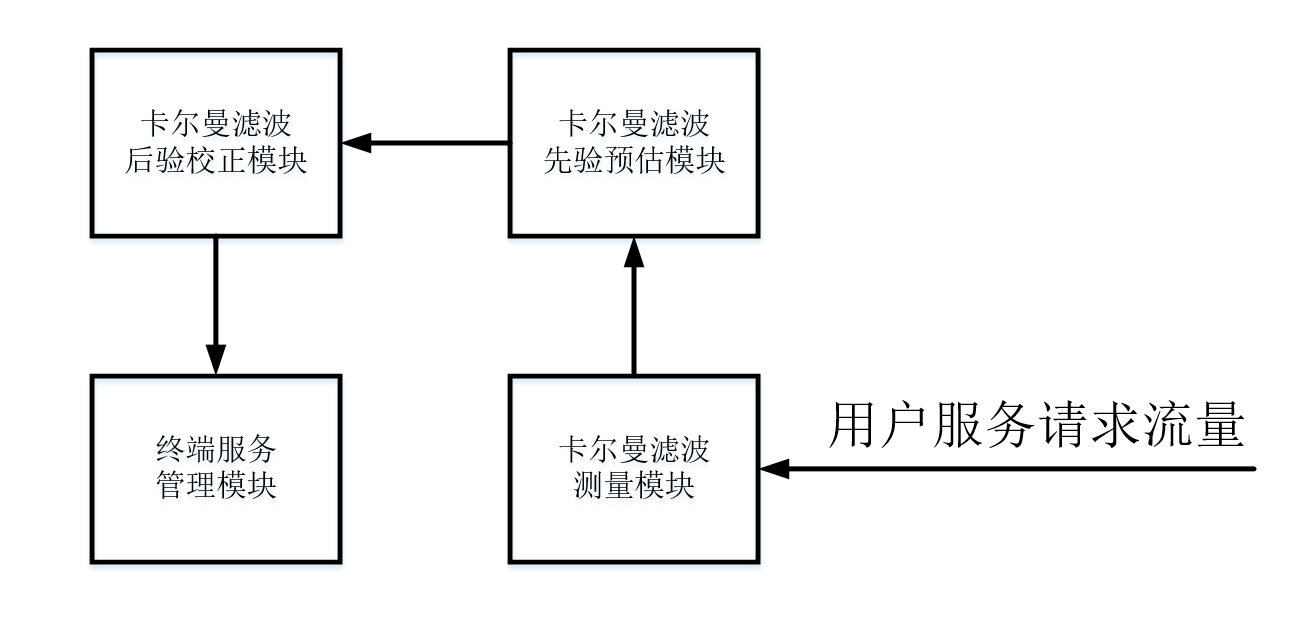
\includegraphics[width=1\linewidth]{Elastic_Service_System_temp}\hfill\\[0.5cm]
  \caption{基于预测的容器弹性服务模块图}
  \label{fig:elastic_service_system}
\end{figure}

针对基于容器化多终端协同服务场景的中的容器弹性服务问题,可以建立如下模型:
\begin{itemize}
    \item 用户服务请求数量预测算法的采样间隔为$T$
    \item 目标服务的单个任务执行时间为$t_x$
    \item 每个容器的最大并发执行任务数量为$K$
    \item \emph{t}时刻正在执行中的任务数量为$m_t$
    \item \emph{t}时刻的终端服务容器数量为$M_t$
    \item \emph{t}时刻新收到的用户服务请求数量为$n_t$
\end{itemize}

在基于容器化多终端协同服务场景中,单一终端计算资源比较有限,虽然有一定并发计算能力,但相比云端服务的并发计算能力仍然差了很多。
为了在保证终端服务用户体验的情况下能够对终端资源更加合理地进行利用,本小节对于多终端协同服务的容器部署策略提出如下需求:
\begin{itemize}
    \item 在保证终端服务用户体验的前提下,尽量减少容器服务规模的变动。
    \item 当存在容器没有执行任何计算任务的时候,关闭该容器并回收资源。
    \item 新的计算任务优先分配给空的容器执行,尽量减少并发。
    \item 当待执行计算任务总数量超过所有容器最大并发能力时,扩展容器服务规模,增加新的可用容器。
\end{itemize}

综合上述问题模型与需求,本小节提出基于改进卡尔曼滤波预测方法的容器弹性服务的部署策略如算法\ref{alg:elastic_service}所示。

\begin{algorithm}
    % \setstretch{1.35}
    \caption{基于预测的容器弹性服务部署策略}
    \label{alg:elastic_service}
    
    \begin{algorithmic}[1]
    \State  开始
    \State  设置问题参数如$T,t_x,K$等
    \While {系统正常运行}
        \State 对$t$时刻用户服务请求数量$n_t$进行采样测量
        \State 根据$n_t$分配任务执行容器,计算$t$时刻的执行中任务数量$m_t$%和终端服务容器数量$M_t$
        \State 预测$t+1$时刻的执行中任务数量为$m_{t+1}=(m_t+n_t)*\frac{T}{t_x}$
        \State 根据$t$时刻测量值及相关参数,利用改进的卡尔曼滤波对$t+1$时刻用户服务请求数量$n_{t+1}$进行预测
        \If{$\frac{m_{t+1}+n_{t+1}}{M_t}>K$}
            \State 调整$t+1$时刻终端服务容器数量为$M_{t+1}=\frac{m_{t+1}+n_{t+1}}{K}$
        \Else
            \If {$\frac{m_{t+1}+n_{t+1}}{M_t}<1$}
                \State 调整$t+1$时刻终端服务容器数量为$M_{t+1}=m_{t+1}+n_{t+1}$
            \Else
                \State 维持$t+1$时刻终端服务容器数量不变$M_{t+1}=M_{t}$
            \EndIf
        \EndIf
        \State 进入$t+1$时刻
    \EndWhile
    
    \end{algorithmic}
    
\end{algorithm}

如算法\ref{alg:elastic_service}所示,在系统开始运行的时候,设置好系统参数,如采样间隔$T$,任务预计执行时间$t_x$,每个容器允许的最大并发计算数量$K$等等。在$t$时刻对用户服务请求数量$n_t$进行采样测量,并且根据相关参数,利用改进的卡尔曼滤波预测算法对$t+1$时刻的用户服务请求数量$n_{t+1}$进行预测。另外还需要对$t$时刻所收到的实际用户服务请求分配到$M_t$个终端服务容器中进行执行,计算$t$时刻执行中的任务数量$m_t$,并且根据$m_t$对$t+1$时刻新的用户流量请求到达前还在执行中的任务数量$m_{t+1}$进行预测。本小节中提出的容器弹性服务部署策略根据采样周期$T$和任务预计执行时间$t_x$来进行预测,预测公式如公式\ref{equ:m_t_1}所示。
\begin{equation}\label{equ:m_t_1}
    m_{t+1}=(m_t+n_t)*\frac{T}{t_x}
\end{equation}
当$\frac{m_{t+1}+n_{t+1}}{M_t}>K$时,算法预计$t+1$时刻新到的用户服务请求数量与正在执行中的任务数量之和将会超过当前所有服务容器所能承受的最大并发数量,所以需要提前将容器服务规模扩展到$M_{t+1}=\frac{m_{t+1}+n_{t+1}}{K}$。当$\frac{m_{t+1}+n_{t+1}}{M_t}<1$时,算法预计$t+1$时刻新到的用户服务请求数量与正在执行中的任务数量之和将会少于当前所有服务容器的数量,也就是预计$t+1$时刻将会出现没有任务可以执行的空闲容器,所以需要在下一时刻到来之前将容器服务规模缩减到$M_{t+1}=m_{t+1}+n_{t+1}$。如果以上两种情况都未发生,即算法预计$t+1$时刻新到的用户服务请求数量与正在执行中的任务数量之和将会正好处于当前服务容器所能够承受的范围内,为了减少并发以及减少容器服务规模的变动次数,算法选择维持服务容器的数量不变。

% 在这个模型里,还需要考虑一下,流量变化到什么程度才能进行扩容缩容,而不是一有变化就调整

% 加个流程图

\section{实验结果}\label{sec:elastic_service_experiment_results}

使用卡尔曼滤波器对用户服务请求数量进行滤波和预测,并同ARMA预测模型进行对比,仿真结果如图\ref{fig:elastic_service_kalman_filter}所示。

\begin{figure}[!htbp]
    \centering
    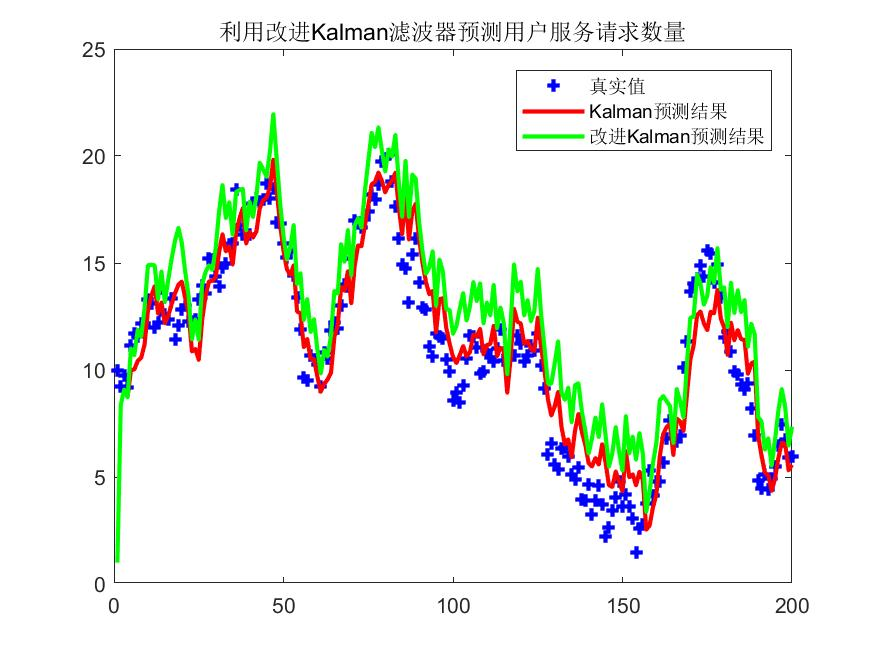
\includegraphics[width=1\linewidth]{kalman_filter}\hfill
  \caption{改进Kalman滤波器预测用户服务请求趋势}
  \label{fig:elastic_service_kalman_filter}
\end{figure}

从图\ref{fig:elastic_service_kalman_filter}中可以看出,相比传统的ARMA模型,使用卡尔曼滤波器对用户服务请求数量的预测更加接近真实值,对于进一步通过用户流量请求数量弹性调整容器服务规模更加有效。而相比原始的卡尔曼滤波器,改进后的卡尔曼滤波器对于增长的用户请求数量更加敏感,能够做出迅速的反应,这也有助于优化基于改进的卡尔曼滤波预测算法的容器弹性服务部署策略的预测效果。

使用基于ARMA预测算法和基于改进的卡尔曼滤波预测算法的容器弹性服务部署策略对容器服务的规模进行动态调整,仿真结果如图\ref{fig:elastic_service_num}所示。

\begin{figure}[!htbp]
    \centering
    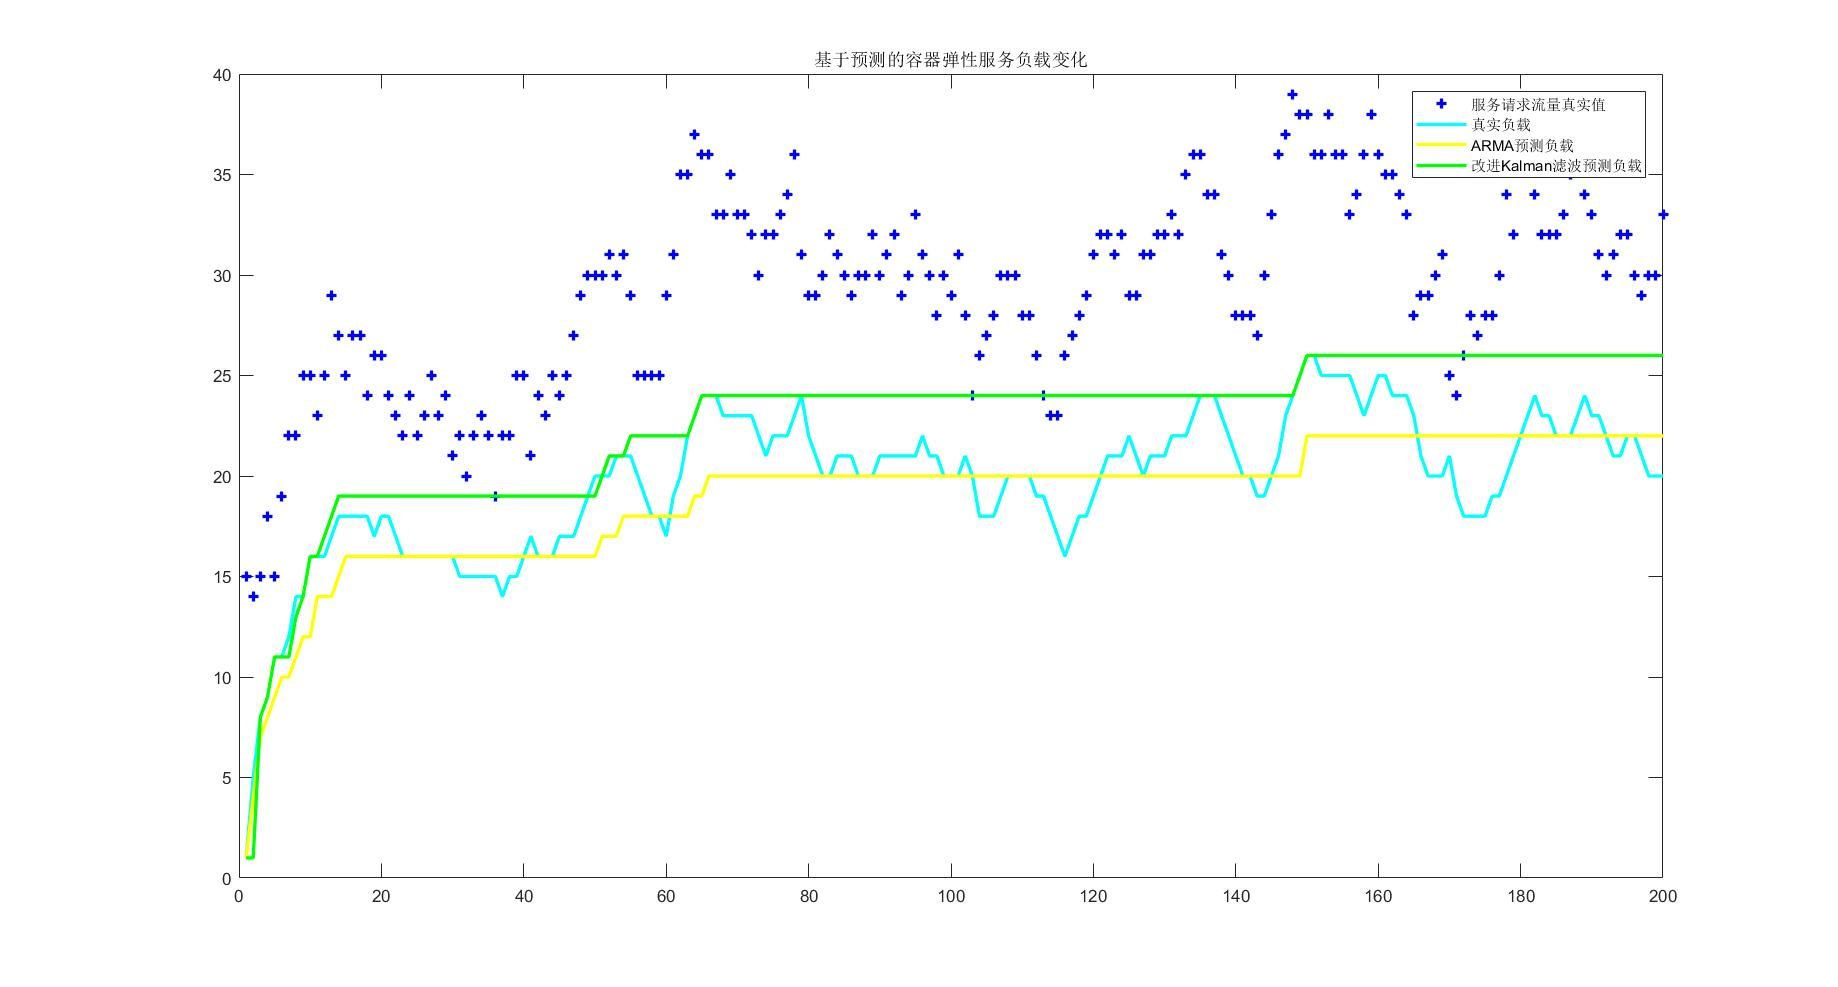
\includegraphics[width=1\linewidth]{elastic_service_num}\hfill
  \caption{基于预测的容器弹性服务负载变化}
  \label{fig:elastic_service_num}
\end{figure}

从图\ref{fig:elastic_service_num}中可以看出,所提出的基于预测的容器弹性服务部署策略能够有效跟随真实负载的变化,在用户服务请求数量增长的时候,所提出的策略能够迅速跟随这种变化,动态扩展容器服务规模,当用户服务请求数量减少的时候,所提出的策略出于减少并发以及减少容器服务规模的变动次数的目的,能够维持容器服务规模不变。相比于基于ARMA算法的部署策略,基于改进卡尔曼滤波预测算法的容器弹性服务部署策略的调整情况更加准确,使得因为策略调整不当而出现的执行任务数量超过容器所能承受最大并发数量的情况明显减少,提高了终端资源利用率,提高了用户体验。

\section{本章小结}\label{sec:elastic_service_summary}

为了解决多终端协同服务技术中的预部署问题,促进提高终端资源利用率和降低用户服务请求响应等待时间之间的平衡,本章提出了基于预测的容器弹性服务策略。基于卡尔曼滤波器,结合多终端协同服务的特点,提出了一种改进卡尔曼滤波算法。根据预测结果提前弹性部署容器服务,动态调整多终端协同服务的规模,平衡提高终端资源利用率与降低用户服务请求响应等待时间之间的关系。